\title{\bf Lecture 8 - Ethereum\\}
\author{\bf Rylan Schaeffer and Vincent Yang\\}
\date{\bf \today \\}

\documentclass{article}
\renewcommand{\thesubsection}{\thesection.\alph{subsection}}
\usepackage{enumerate}
\usepackage{listings}
\usepackage{amsmath}
\usepackage{graphicx}
\setlength{\oddsidemargin}{0in}
\setlength{\evensidemargin}{0in}
\setlength{\textheight}{9in}
\setlength{\textwidth}{6.5in}
\setlength{\topmargin}{-0.5in}

\begin{document}
\maketitle

Note: This lecture is based on Princeton University's BTC-Tech: Bitcoin and Cryptocurrency Technologies Spring 2015 course.

\section*{What is Ethereum}
\begin{itemize}
  \item Why the name Ethereum?
    \subitem It's a metaphor referring to ether, the hypothetical invisible medium that permeates the universe and allows light to travel
  \item The old way: You send a message, the message goes through servers, the server sends to client
  \item The new way: You send a message, the messsage goes to a set of independent computers all over the world, but nobody can access the full message
    The message is delivered
    \subitem Every computing computer is compensated for work
  \item Computer owners want to monetize their work and sell ether for real dollars, dApp developers need Ether to run their apps on the network and want to by ETH
    for real dollars
  \item Since blockchain is public, we want privacy for users
\end{itemize}

\section*{History and Motivations}
\begin{itemize}
  \item Alternative decentralized ledger protocol, not an alternative cryptocurrency
  \item In late 2013, Vitalik Buterin published the Ethereum white paper, and later formally announces it at the North American Bitcoin Conference in early 2014
    \subitem He researched and worked in the Bitcoin community
  \item Vitalik Buterin works with Dr. Gavin Wood to co-found Ethereum. In April 2014, Gavin published the Ethereum Yellow Paper
    \subitem Whitepaper is summary, Yellowpaper is formal paper of research (longer)
    \subitem Through the instructions of the yellow paper, the Ethereum client has been implemented in 7 languages: C++, Go, Python, Java, Javascript, Haskell, Rust)
  \item You need a large bootstrapping effort to assemble resources needed to get it up and running, so they kickstarted a large network of developers, miners, investors,
    and other stakeholders via. a presale of Ether tokens, the currency unit of Ethereum
  \item In July 2014, Ethereum distributed original allocation of Ether via. 42-day public ether presale, netting 31,591 Bitcoins, worth 18,439,086 at the time, in exchange
    for 60,102,216 ether
    \subitem This was used to pay legal debts and for developer effort
  \item Olympic: In 2014 and 2015 they hosted a set of proof of concept releases through a testnet called Olympic. The dev community was invited to test the limits of the network
    with prize rewards on those with records, or successfully breaking the system in one way or another
  \item Bounty Program: Early 2015, they offer BTC rewards for finding vulnerabilities. This is still active
  \item Ethereum Frontier Network launched on July 30th, 2015 where developers started writing smart contracts to deploy on the network, and miners started to join
    to help secure the blockchain and earn ether from mining blocks
    \subitem This was the first milestone and was to be a beta version, but was much more capable/reliable than anyone expected, so more people rushed to join
  \item Feb 6, 2016: First Ethereum Browser - this hosts DApps, or Decentralized Apps, where you can 
    \begin{enumerate}
      \item Transfer ownership of property
      \item Issue a local currency (transaction)
      \item Create marriage contracts
      \item Create business contracts
      \item Create rental contracts
      \item Transfer Money
      \item Buy Insurance
      \item Vote
      \item Verify information
      \item Take out a loan, etc.
    \end{enumerate}
\end{itemize}

\section*{Bitcoin vs. Ethereum}
\begin{itemize}
  \item Bitcoin is a stack-based language
  \item Ethereum is a Turing-Complete language
  \item Turing Complete vs. Stack Based: (Automata Theory)
    \begin{itemize}
      \item Stack Based means it relies on a stack machine model for passing parameters
        \subitem e.g. push 2, push 4, mult
        \subitem e.g. XML, HTML, JSON, Script (Bitcoin)
      \item Turing Complete means it can do anything a Turing Machine can.
      \item On a basic sense, for imperative languages, Turing Complete has to have:
        \begin{enumerate}
          \item Needs a form of conditional repetition or jump
          \item A way to read and write some form of storage (variables, tape) (with infinite space or dynamically allocated)
          \item e.g. Java, C++, Python, etc.
          \item Imperative means it uses statements to change state. The alternative would be lambda-calculus based functional programming.
        \end{enumerate}
    \end{itemize}
  \item Transactions confirmed in seconds compared to minutes for Bitcoin
  \item Difference is purpose:
    \subitem Bitcoin is an alternative to regular money, while Ethereum is a platform
    that facilitates peer to peer contracts and applications via its own currency vehicle.
  \item Market cap of Ether is more than Ripple and Litecoin, but far behind Bitcoin
\end{itemize}

\section*{How it Works}
\begin{itemize}
  \item 3 Tier Architecture:
    \begin{enumerate}
      \item Advanced Browser as the client
      \item Blockchain Ledger as shared resource
      \item Virtual Network of Computers
    \end{enumerate}
  \item Sandwich Complexity Model:
    \subitem Bottom architecture and Top interfaces should be simple and understandable
    \subitem Where complexity is inevitable, push into the middle
  \item Specialized form of Cloud Computing
\end{itemize}

\section*{Ether (Gas and Fees)}
\begin{itemize}
  \item Ether is to be treated as a ``crypto-fuel'', a token whose purpose is to pay for computation, and is not intended to be used as or considered
    a currency, asset, share or anything else
  \item All transactions in Bitcoin are roughly the same, since they can be modeled to the same unit (BTC).
  \item Since Ethereum is Turing-complete, it needs to take into account
    \subitem cost of bandwidth
    \subitem cost of storage
    \subitem cost of computation
  \item Halting problem cannot be reliably predicted ahead of time
  \item Prevent denial-of-service via infinite loops?
  \item Basic mechanism for transaction fees:
    \begin{itemize}
      \item Every transaction must specify a quantity of ``gas'' that it is willing to consume (\emph{startgas})
        and a fee it is willing to pay per unit gas (\emph{gasprice}). At the start of execution, 
        $startgas\ \cdot gasprice$ ether are removed from the transaction sender's account
      \item All operations, including database reads/writes and computational steps consume gas
      \item If a transaction execution finishes (returns), consuming less gas than needed, then the transaction executes
        and the sender receives a refund of $gas_rem\ \cdot gasprice$ and miner of block receives $(startgas - gas_rem)\ \cdot
        gasprice$
      \item If a transaction runs out of gas, then all execution reverts, but the transaction is valid, and the sum $startgas\ \cdot gasprice$
        is given to the miner
    \end{itemize}
    \subitem Prevents shitty code
  \item Proof of necessity:
    \begin{itemize}
      \item If transaction don't specify a gas limit, then a malicious user could have an infinite loop, but miners can't tell beforehand
      \item Alternative to strict gas-counting, time-limiting doesn't work because it is subjecetive - some machines are faster than others
      \item Entire value $startgas\ \cdot gasprice$ has to be removed at beginning so account doesn't run out half way. 
        \subitem Balance checking isn't enough because the account can send it somewhere else
      \item If execution didn't revert, then contracts need strong security measures to ensure that not only part a program is executed, or else
        some changes in contract execution could be executed but not others
    \end{itemize}
  \item Further features:
    \begin{itemize}
      \item 21000 gas is charged as base fee. This covers sending sender address from signature and disk/bandwith space of storing transaction
      \item Transactions can have unlimited data, so the gas fee is 1 gas per zero byte and 5 gas per nonzero byte (encourage compression)
      \item Memory is infinite, but gas is 1 per 32 bytes of expansion
    \end{itemize}
  \item Economics of Gas Pricing
    \subitem Bitcoin has voluntary fees, relying on miners to act as gatekeeprs.
    \subitem The equivalent is to let senders set arbitrary gas costs. Unfortunately, since
    every transaction a miner includes has to be processed by the network, the vast majority
    of cost of transaction processing is by 3rd parties and not the miner, so tragedy of the commons might occur
    \subitem The solution is a voting system. Miners have the right to set a gas limit to be within
    ~0.0975\% (1/1024) of the gas limit of the gas block, so the gas limit should be around the median of
    miner's preferences. 
    \subitem The hope is that this can be soft-forked into a more precise algorithm
\end{itemize}

\section*{Patricia Trees}
\begin{itemize}
  \item Merkle Trees can let us efficiently prove what happened. However, there are limitations:
    \begin{itemize}
      \item CAN prove inclusion of transactions
      \item CAN'T prove anything about current state
        \subitem e.g. Digital Asset holdings, name registrations, status of financial contracts, etc.
      \item In order to tell anything about the next transaction, you need to know the authenticity
        of every single prior transaction.
    \end{itemize}
  \item Every block header has not 1 Merkle Tree, but 3 trees for 3 kinds of objects:
    \begin{enumerate}
      \item Transactions
      \item Receipts (data showing effect of transaction)
      \item State (Patricia)
    \end{enumerate}
    \subitem This gives capabilities of:
    \begin{enumerate}
      \item Has this transaction been included in a past block?
        \subitem Transaction Tree
      \item Tell me all instances of an event of type X (e.g. crowdfunding contract reaching a goal from this address
        in the past Y time) 
        \subitem Receipt Tree
      \item What is my balance?
        \subitem State Tree
      \item Does this account exist?
        \subitem State Tree
      \item Pretend to run this transaction. What's the output?
        \subitem State Tree, but more complex: 
        \subitem You need a Merkle \emph{state transition proof}
        \subitem Make claim "If you run transaction $T$ on state with root $S$, the result
        will be a state with root $S'$, with log $L$ and output $O$". (Output is the return statement).
        \subitem To do this, the server locally creates a fake block, and pretends to be a light client
        while applying the transaction. It 'responds' to all of its own queries, then keeps track of returned
        data. Then, the server sends the client the combined data. using provided proof as database. If it reaches
        the same result, then it works.
    \end{enumerate}
  \item Patricia Tree:
    \begin{itemize}
      \item Merkle trees are good data structures for transactions, because it doesn't matter
        how much time it takes to edit, since it's created once then forever frozen.
      \item However, the state tree is different. The \emph{State} in \emph{Ethereum} has a key value map, where keys
        are addresses and values are account declarations, listing the balance, nonce, code, and storage for each account.
      \item Unlike transaction history, the state has to be frequently changed - balance and nonce is often changed, and new accounts
        are often made.
      \item We want a data structure 
        \begin{itemize}
          \item Where we can quickly find the new tree root after insert, update edit or delete, without
            recomputing everything.
          \item Depth of tree is bounded, so an attacker can't perform a denial of service attack by making the tree super deep.
          \item Root depends on data, not order.
        \end{itemize}
    \end{itemize}
    \begin{itemize}
      \item Radix Tree + Merkle Patricia Tree modification:
        \begin{itemize}
          \item Given a key/value pair that should be inserted, the key will be split so its sub-parts (e.g. characters and each value) will be
            a node in a tree, so if we want to retrieve a reference value we should jump from node to node representing part of the key
            until we find the end and there we will have the value.
          \item Each node on the diagram has 17 elements which are representing slots for \emph{[0.. f]} digits of encoding, and one more slot - the last one, for the value (if it exists)\\
          \item In our case we will split the key to a nibbles of it's ASCII code:
          \item Let's take $dog$ string as a key, in order to get it's nibbles, we check its ASCII code which is $[\ 0x64\ 0x6f\ 0x67\ ]$, now the nibbles of 
            the key are 4 bits of each byte: $6, 4, 6, f, 6, 7$.
          \item Another example is the key ``do'' which obviously will be encoded to $6, 4, 6, f$. (``dog'' with no ``g'').
          \item Now, let's see how to encode the key value $["do" : "verb"]$ and $["dog" : "puppy"]$ into a data structure: (Diagram 1)
          \item 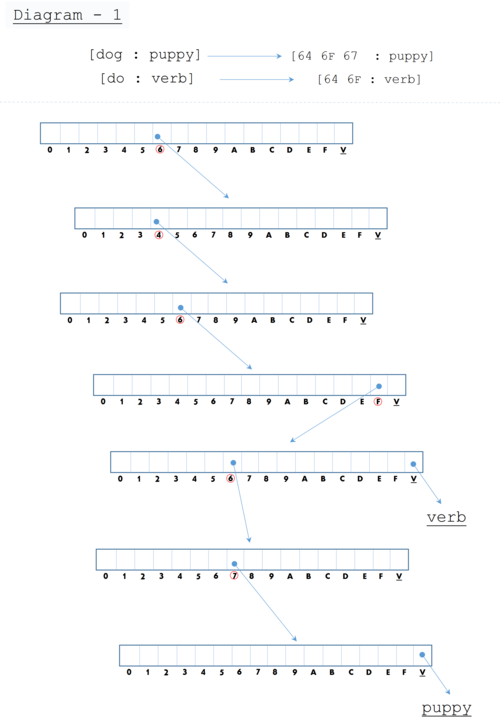
\includegraphics[width=4in]{trie-post-diagram-1.png}
          \item Problem with Radix Trees: You need over a kb to store a key that's a few hundred characters long - very inefficient
          \item How to improve it?? Define a too-long-path
          \item Insert another key/value: \emph{``doggiestan'':``awesome\_place''}. 
          \item 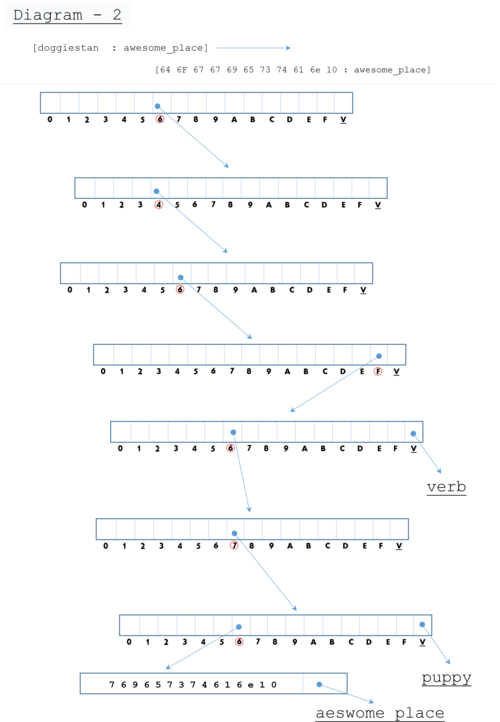
\includegraphics[width=4in]{trie-post-diagram-2.png}
          \item How to encode the finger print? \emph{sha3(root\_node)} function.
          \item 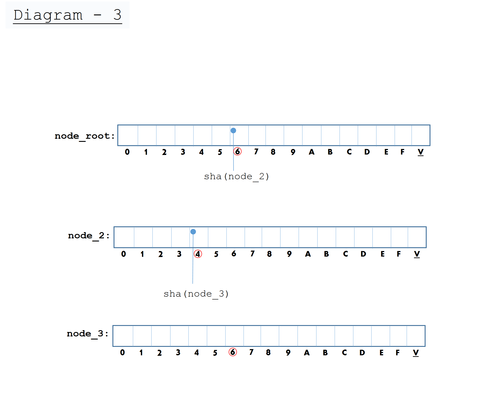
\includegraphics[width=4in]{trie-post-diagram-3.png}
        \end{itemize}
      \item ``Merkle'' part comes from the fact that a cryptographic hash of a node is used as a pointer to a node, rather than a memory location
      \item Fully deterministic - a Patricia tree with the same (key, value) bindings is guaranteed to be exactly the same down to the last byte, with the same
        root hash
      \item O(log(n)) for inserts, lookups, and deletes
      \item The solution: A node in a Merkle Patricia Tree is one of:
        \begin{enumerate}
          \item NULL (empty string)
          \item A two-item array $[key, v]$ (aka kv node)
          \item A 17-item array $[\ v0\ ... v15, vt]$ (aka diverge or branch node)
        \end{enumerate}
        \subitem In the event that there is a long path of nodes, each with only one element, we shortcut the descent by setting
        up a kv node $[key, value]$ where the key is the path to descend, and the value is the hash of the node. 
        \subitem Also, internal nodes can no longer have values, only leaves with no children can
        \subitem To be fully generic, if we want to store ``dog'' and ``doge'' at the same time, we use a terminator symbol to the alphabet
        so you know it's a value.
      \item For a kv node, a two-item array $[key, v]$, $v$ can be a value or a node.
        \subitem When $v$ is a value, the key must end with the terminator
        \subitem When $v$ is a node, the key must not have a terminator
      \item http://ethereumj.io/blog/2015/07/05/Ethereum-Trie/
    \end{itemize}
  \item Given the 3 types of nodes, let's say we have a tree with the pairs \emph{(``dog'', ``puppy''), (``horse'', ``stallion''), (``do'', ``verb''), (``doge'', ``coin'')}.
    \subitem Convert this to hex:
    \begin{lstlisting}
    [ 6, 4, 6, 15, 16 ] : 'verb'
    [ 6, 4, 6, 15, 6, 7, 16 ] : 'puppy'
    [ 6, 4, 6, 15, 6, 7, 6, 5, 16 ] : 'coin'
    [ 6, 8, 6, 15, 7, 2, 7, 3, 6, 5, 16 ] : 'stallion'
    \end{lstlisting}
    \subitem Build the tree:
    \begin{lstlisting}
    ROOT: [ '\x16', A  ]
    A:['', '', '', '', B, '', '', '', C, '', '', '', '', '', '', '', '']
    B:['\x00\x6f', D  ]
    D:['', '', '', '', '', '', E, '', '', '', '', '', '', '', '', '', 'verb']
    E:['\x17', F  ]
    F:['', '', '', '', '', '', G, '', '', '', '', '', '', '', '', '', 'puppy']
    G:['\x35', 'coin']
    C:['\x20\x6f\x72\x73\x65', 'stallion']
    \end{lstlisting}
  \item 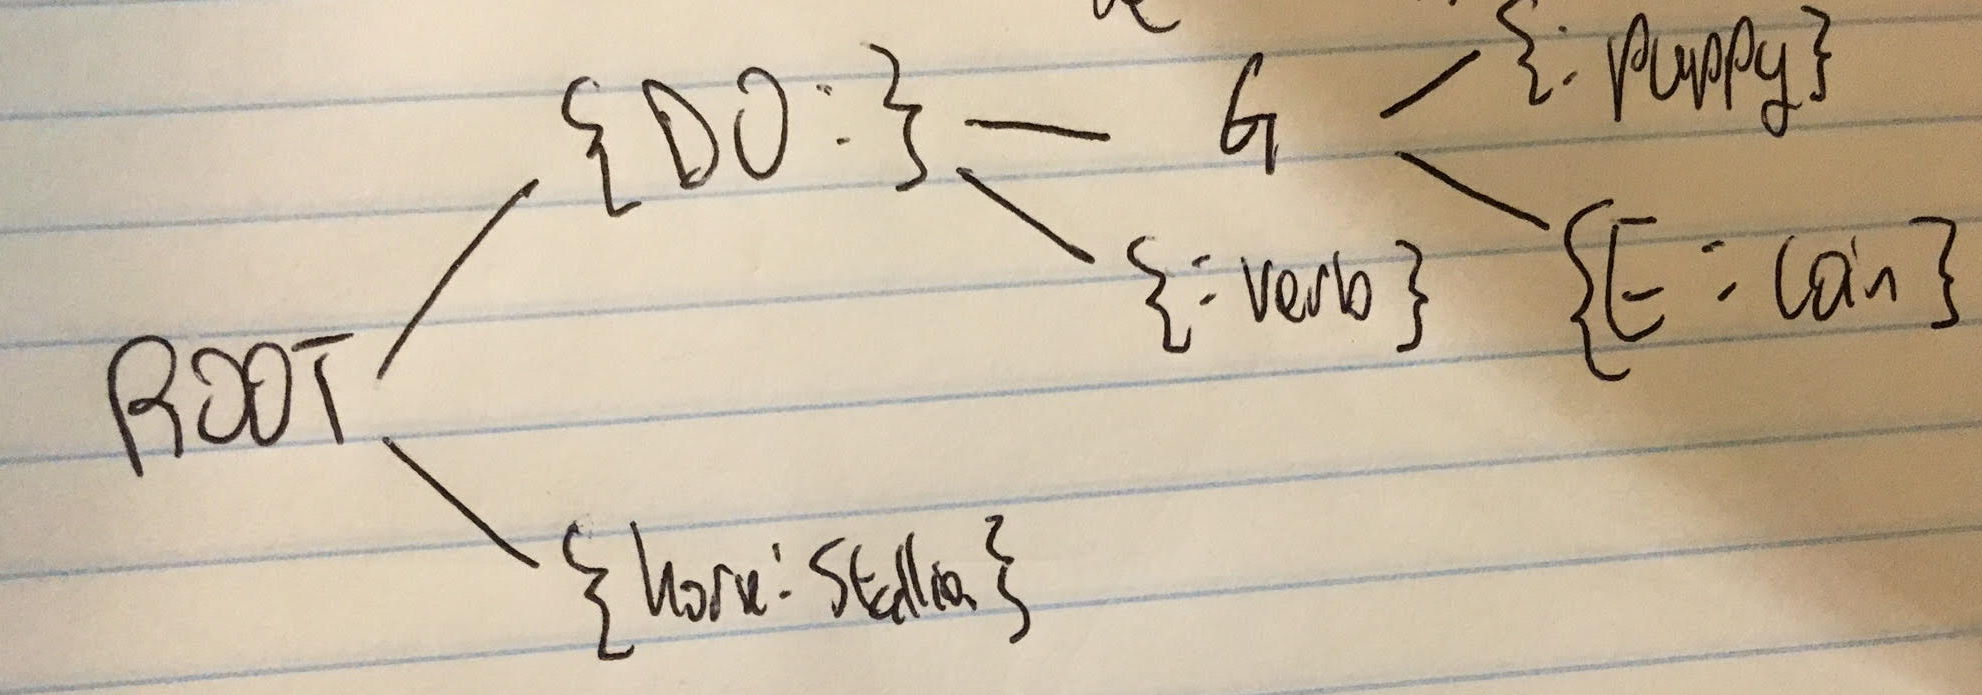
\includegraphics[width=4in]{patriciaex.png}
\end{itemize}

\section*{SHA-2 vs. SHA-3}
\begin{itemize}
  \item Bitcoin uses HashCash, which uses SHA-256, which is in the SHA-2 family. 
  \item SHA-2's predecessors were HD5 and SHA-1, which were broken. NIST (National Institute of Standards and Technology) decided to start creating a replacement for SHA-2, 
    but SHA-2 turned out to be surprisingly robust
  \item Regardless, Ethereum uses SHA-3
\end{itemize}

\section*{Mining}
\begin{itemize}
  \item A block is only valid if it contains Proof of Work of a given difficulty
    \subitem In Ethereum 1.1, this is likely going to be switched for a proof of stake model
  \item The proof of work used is called Ethash, which is memory hard
    \subitem This way, it is ASIC resistant
    \subitem This is achieved with a POW algorithm that requires choosing subsets of a fixed resource dependent on the nonce and block header.
    \subitem This resource is called a DAG. 
    \subitem Solve a contraint on a subset of the DAG, but has large memory requirements with little super-linear benefit. This is such that pooling has no advantage
    \subitem Currently CPUs are basically worthless, GPU's are dominant
  \item Difficulty is set such that every 12 seconds, there is a new block
  \item Successful PoW miner receives 
    \subitem static block reward of 5.0 Ether
    \subitem All gas expended within the block, or all gas consumed by execution of all transactions in the block submitted by winner for miners. Over time, this should
    dwarf the static award
    \subitem Extra reward for including Uncles of the block, in the form of 1/32 per Uncle included
  \item Uncles are stale blocks, and are rewarded to neutralize effect of network lag on dispersion of mining rewards, to increase security
    \subitem Receive 7/8 of static block reward, max of 2 uncles per block
\end{itemize}

\section*{Casper - Proof of Stake}
\begin{itemize}
  \item Security deposit based concensus protocol - Nodes, called bonded validators, have to place a security deposit (bonding) to serve consensus
  \item https://blog.ethereum.org/2015/08/01/introducing-casper-friendly-ghost/
\end{itemize}

\section*{Light Clients}
\begin{itemize}
  \item Let users in low-capacity environments maintain assurance/use some features
  \item Know the state of an account at some time
  \item Check transaction confirmation
  \item Download a subset of information, no mining
\end{itemize}


\section*{UTXO vs. Accounts}
https://github.com/ethereum/wiki/wiki/Design-Rationale


\end{document}
